% spectral domain
\subsection{Scattering angle -- resolution length relation}

While radiation patterns characterize scattering for point perturbations, they 
can be generalized to arbitrary perturbations that fit into the Born 
approximation. If the scattering experiment is handled in the model wavenumber domain \citep{devaney1984}, then
we can access additional features of the scattering such as resolution (\figref{ksg}).
%
For acoustic monochromatic plane waves, there is a simple relation between 
the wavenumbers in the model and the scattering angles \citep{ewald1969,devaney1984}. 
\cite{wu:11} compared wavenumbers that are covered by scattered waves in vertical seismic profiling (VSP) 
and surface observations. \cite{mora1989} analyzed the contributions of reflections to the illuminated wavenumber spectrum in background media. \cite{kazei2013gp} 
provided a quantitative wavenumber illumination analysis of the spectrum covered by head waves and diving waves. \cite{podgornova,podgornova2018} analyzed 
the resolvability of elastic parameter spectra in elastic VTI media. 
\cite{kazei2018} presented spectral coverage and resolution for orthorhombic 
parameters. 
%
\begin{figure}
	\centering
	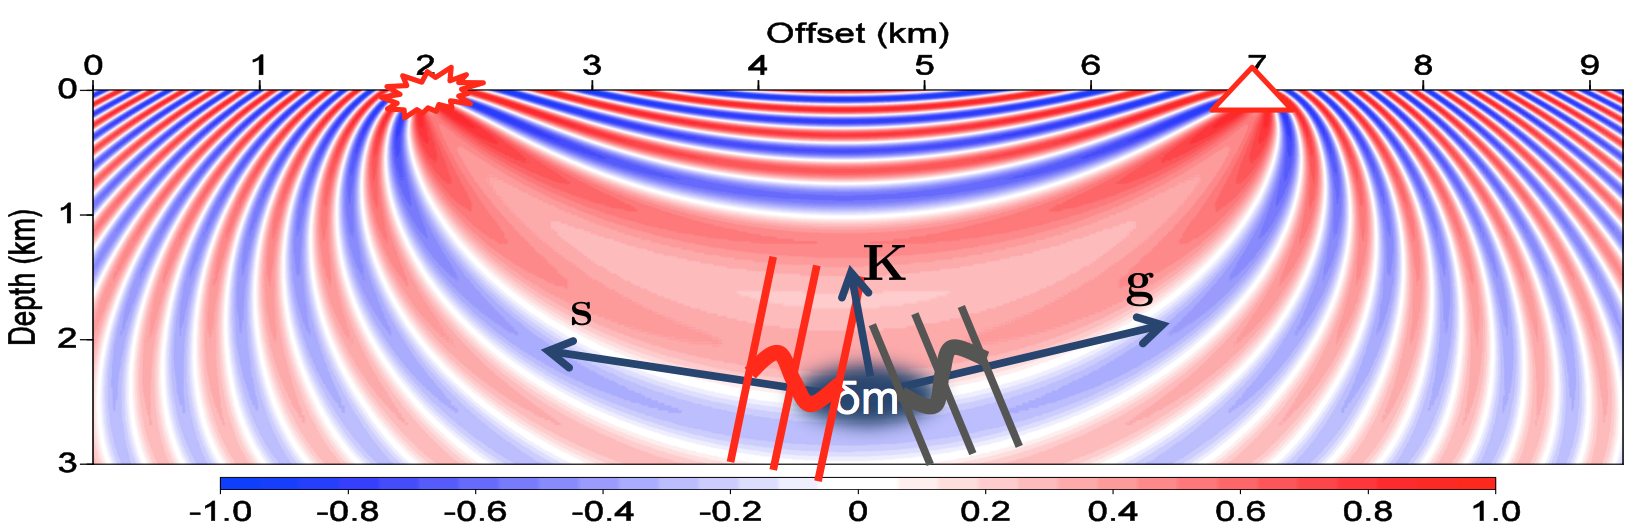
\includegraphics[width=0.9\linewidth]{Fig/Ksg}
	\caption{Sensitivity kernel for a single source-receiver pair for FWI in the frequency domain in a linearly increasing velocity background \citep{alkhalifah2014scattering,kazei2016}. Source is indicated as an explosion and receiver as a triangle. On the wide red wavepath of diving wave the update can only be smooth, wavenumbers in the gradient  $\Kv = \omega(\sv+\gv)$ are very small. With a decrease in the scattering angle (the angle between slowness vectors towards the source $\sv$ and receiver $\gv$), the resolution length $L \propto |\Kv|^{-1}$ also decreases, which results in more wiggly structure of the gradient away from the wavepath.}
	\label{fig:ksg}
\end{figure}

In our previous work \citep{kazei2018}, we performed an analysis of the 
radiation patterns describing the scattering of $P$ waves on orthorhombic 
parameters in an isotropic, homogeneous-medium background. We present a similar 
analysis for different types of scattering. Namely, we consider $S$ waves and 
$P-S$ conversions. In order to access the scattering caused by isotropic and VTI 
parameter perturbations, we use a hierarchical parameterization based on that of 
\cite{juwon2016, kazei2018}.